\documentclass[../Funzionalita.tex]{subfiles}

\begin{document}

\subsection{Localizzazione utente}
\label{subsec:LocalizzazioneUtente}
		
		\subsubsection{Panoramica}
			L'applicazione offre la funzionalità di localizzare l'utente all'interno di un edifico in cui risiedono i beacon riconosciuti dall'applicazione e di mostrare semplici informazioni sull'edifico.
			
			La localizzazione utente avviene seguendo le seguenti fasi:
			\begin{enumerate}
				\item l'utente avvia l'applicazione;
				\item l'applicazione avvia il monitoring per poter rilevare i beacon circostanti;
				\item l'applicazione avvia il ranging e reperisce l'identificativo major dei beacon;
				\item l'applicazione si accerta che i beacon rilevati siano pertinenti all'applicazione attraverso un confronto tra major rilevato e major dei beacon nel database locale;
				\item se il beacon è riconosciuto ed esiste un match nel database locale:
					\begin{itemize}
						\item vengono costruiti concretamente gli oggetti dai dati nel database locale e raccolti nell'oggetto \BuildingMap;
						\item vengono mostrate all'utente informazioni sull'edificio in cui si trova;
					\end{itemize}
				%\item se il beacon è riconosciuto e non esiste un match nel database locale:
					%\begin{itemize}
						%\item viene segnalato all'utente che la mappa dell'edificio non è scaricata nel device;
						%\item l'utente se lo desidera è reindirizzato alla gestione delle mappe;
					%\end{itemize}
				%\item se il beacon non è riconosciuto:
					%\begin{itemize}
					%	\item viene ignorato.
					%\end{itemize}
			\end{enumerate}
			
		\newpage
		\subsubsection{Interfaccia grafica}
			\HomeViewImp\ implementa la vista principale che viene visualizzata subito dopo l'avvio dell'applicazione dopo la generazione della splash page da \MainActivity\ la classe di avvio dell'applicazione. \HomeView\ è legata alla componente del presenter \HomeActivity\ e può essere di due tipologie:
			\begin{itemize}
				\item vuota, ossia priva di informazioni dell'edificio. Ciò significa che il device non ha ancora rilevato un beacon riconosciuto dall'applicazione.
				\item mostra le informazioni dell'edificio in cui è l'utente. Ciò significa che l'applicazione ha rilevato almeno un beacon riconosciuto dall'applicazione.
			\end{itemize}
		
			\paragraph*{Componenti interne}
			\begin{itemize}
			
				\item Package:
				\begin{itemize}
					\item[] \view;
				\end{itemize}
				
				\item Interfacce e classi:
				\begin{itemize}
					\item[] \HomeView, \HomeViewImp;
				\end{itemize}
				
			\end{itemize}
			
			\paragraph*{Componenti esterne}
			\begin{itemize}
				\item Interfacce e classi SDK:
				\begin{itemize}
					\item[] \Activity, \Toolbar, \TextView, \DrawerLayout, \TextView, \SearchView, \FloatingActionButton, \ListView, \ActionBarDrawerToggle.
				\end{itemize}
			\end{itemize}
			
			Nella figura \ref{fig:LocalizzazioneUtente-HomeView} si indicano i seguenti widget offerti dal kit Android SDK:
				\begin{enumerate}
					\item \SearchView;
					\item \TextView;
					\item \ListView;
					\item \FloatingActionButton.
				\end{enumerate}
			

				\begin{figure}[h]
					\centering
					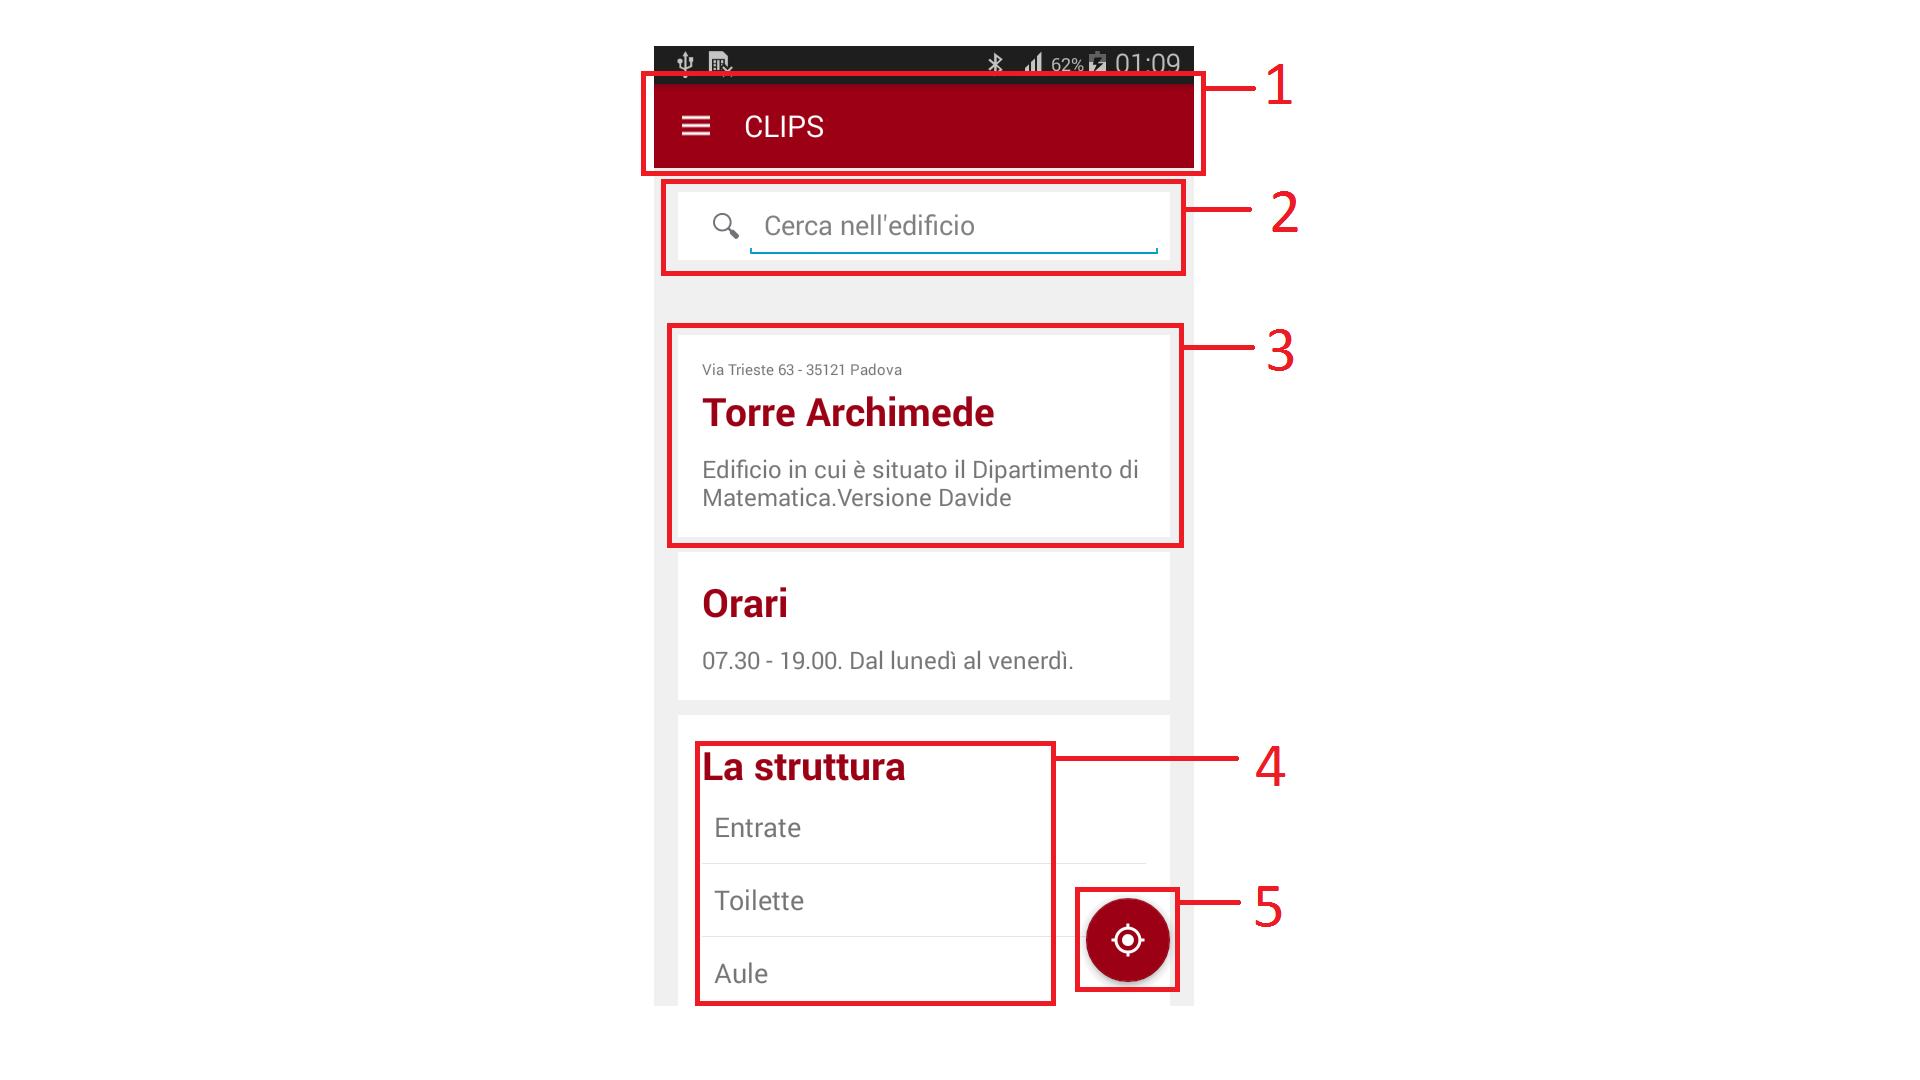
\includegraphics[width=\textwidth]{img/LocalizzazioneUtente-HomeView_}
					\caption{HomeView - Screen con informazioni edificio}
					\label{fig:LocalizzazioneUtente-HomeView}
				\end{figure}
				
				%\begin{figure} [h]
					%\centering
					%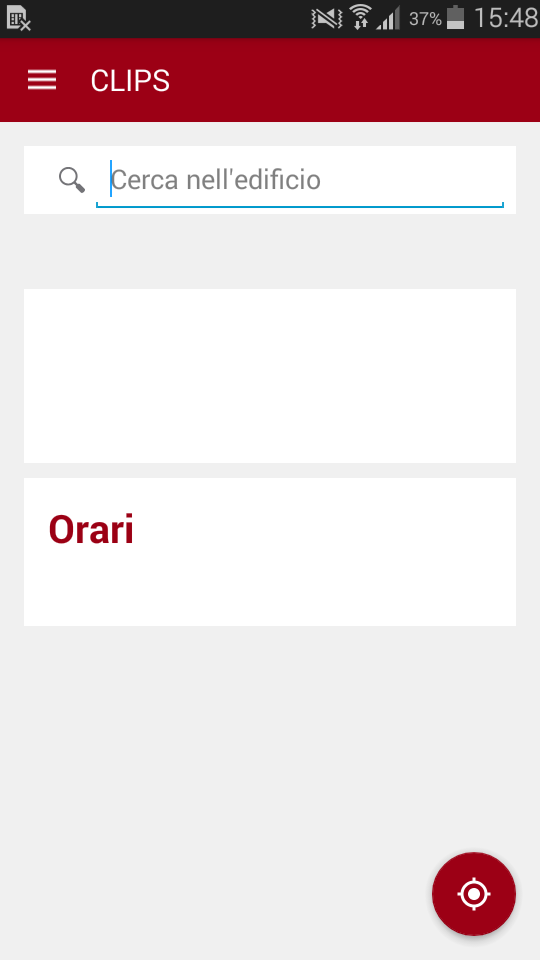
\includegraphics[scale=0.19]{img/LocalizzazioneUtente-HomeView2}
					%\caption{HomeView - Screen vuota}
					%\label{fig:LocalizzazioneUtente-HomeView2}
				%\end{figure}
				
				
			

		\newpage	
		\subsubsection{Presenter}
			Il compito del presenter per questa funzionalità è affidato all'oggetto \HomeActivity\ che comunica con la vista \HomeViewImp\ attraverso l'interfaccia \HomeView. \HomeActivity\ comunica con le componenti del model \InformationManager\ attraverso la dependency injection.
		
			\paragraph*{Componenti interne}
			\begin{itemize}
			
				\item Package:
				\begin{itemize}
					\item[] \view;
					\item[] \presenter;
				\end{itemize}
				
				\item Interfacce e classi:
				\begin{itemize}
					\item[] \HomeActivity, \HomeView;
				\end{itemize}
				
			\end{itemize}
			
			
			\paragraph*{Componenti esterne}
			
			\begin{itemize}
				\item Interfacce e classi SDK:
				\begin{itemize}
					\item[] \Activity, \InformationManager.
				\end{itemize}
			\end{itemize}
			
			
		\subsubsection{Rilevamento beacon}
			La classe \BeaconManagerAdapter\ estende un bind \Service\ (vedi appendice \ref{sec:FondamentiDiAndroid}) ed ha il compito di effettuare il ranging e il monitoring dei beacon circostanti. Il ranging è l'operazione svolta in background per riconoscere i beacon circostanti senza eccessiva precisione mentre il monitoring è l'operazione che segue in cui i beacon vengono invece rilevati con tutte le informazioni e con più precisamente.
			La comunicazione dei beacon rilevati dal \model\ avviene attraverso l'uso degli oggetti \MyBeacon\ inviati tramite \Intent\ per cui serializzati. Gli \Intent\ vengono recuperati tramite \BroadcastReceiver\ implementato in altre classi.
			
			\paragraph*{Componenti interne}
			\begin{itemize}
			
				\item Package:
				\begin{itemize}
					\item[] \model;
					\item[] \beacon;
				\end{itemize}
				
				\item Interfacce e classi:
				\begin{itemize}
					\item[] \BeaconManagerAdapter, \MyBeacon, \MyBeaconImp, \MyDistanceCalculator, \LocalBinder, \BeaconRanger;
				\end{itemize}
												
			\end{itemize}
			
			\paragraph*{Componenti esterne}
			\begin{itemize}
			
				\item Interfacce e classi AltBeacon:
				\begin{itemize}
					\item[] \BeaconManager, \BootstrapNotifier, \BeaconConsumer, \RangeNotifier, \Region, \BeaconParser, \DistanceCalculator, \Beacon;
				\end{itemize}
			
				\item Interfacce e classi JDK:
				\begin{itemize}
					\item[] \PriorityQueue;
				\end{itemize}
				
				\item Interfacce e classi SDK:
				\begin{itemize}
					\item[] \Intent, \LocalBroadcastManager, \Service, \Binder, \LocalBroadcastManager, \IBinder.
				\end{itemize}
				
				
				
			\end{itemize}
			
			
		\subsubsection{Costruzione BuildingMap}
			L'oggetto \InformationManagerImp\ comunica a \DatabaseService\ la necessità di costruire l'oggetto \BuildingMap. \DatabaseService\ costruisce tale oggetto incaricando \PointOfInterestService, \RegionOfInterestService, \EdgeService, \PhotoService di costruire le componenti di \BuildingMap ossia:
			\begin{itemize}
				\item \PointOfInterest;
				\item \RegionOfInterest;
				\item \EnrichedEdge;
			\end{itemize}
			Tali componenti sono prelevate e costruite facendo uso di semplici oggetti data grazie alle classi con suffisso \textit{Dao}. Questi oggetti semplici sono descritti da un nome riferito all'elemento all'interno di una tabella del database locale e con il suffisso \textit{Table}. 
			Le operazioni eseguite per costruire \BuildingMap\ si distinguono in due casi:
			\begin{itemize}
				\item I dati necessari per la costruzione di \BuildingMap\ sono nel database locale. A questo punto se la versione dei dati in locale corrispondono alla versione in remoto l'\InformationManagerImp\ incarica \DatabaseService\ di costruire l'oggetto \BuildingMap\ come spiegato in precedenza, altrimenti si effettuano le operazioni descritte nel caso successivo;
				\item I dati necessari per la costruzione di \BuildingMap\ devono essere scaricati dal database remoto. A questo punto, dopo aver fatto richiesta all'utente di poter effettuare il download dei dati, \DatabaseService\ reperisce le informazioni dal database remoto converte i dati dal formato Json trasmetto ad oggetti attraverso le classi con prefisso \textit{Remote}, inserisce tali oggetti nel database locale attraverso le classi con suffisso \textit{Dao} e infine costruisce l'oggetto \BuildingMap\ desiderato.
			\end{itemize}
			
		
			\paragraph*{Componenti interne}
			\begin{itemize}
			
				\item Package:
				\begin{itemize}
					\item[] \model
					\item[] \dataaccess
					\item[] \service
					\item[] \dao
					\item[] \graph
					\item[] \edge
					\item[] \vertex
					\item[] \area
				\end{itemize}
				
				\item Interfacce e classi:
				\begin{itemize}
					\item[] \BuildingMap, \BuildingMapImp, \BuildingInformation, \PointOfInterest, \RegionOfInterest, \EnrichedEdge, \DatabaseService, \BuildingService, \EdgeService, \PhotoService, \PointOfInterestService, \RegionOfInterestService, \ServiceHelper,
					\CursorConverter, \DaoFactoryHelper, \RemoteDaoFactory, \SQLiteDaoFactory;
					
					\item[] con suffisso \textit{Dao}: 
					\SQLDao, \BuildingDao, \CategoryDao, \EdgeDao, \EdgeTypeDao, \PhotoDao, \PointOfInterestDao, \RegionOfInterestDao, \RoiPoiDao, \RemoteBuildingDao, \RemoteCategoryDao, \RemoteEdgeDao, \RemoteEdgeTypeDao,  \RemotePhotoDao,  \RemotePointOfInterestDao, \RemoteRegionOfInterestDao, \RemoteRoiPoiDao;
					
					\item[] con prefisso \textit{SQL} e suffisso \textit{Dao}:
						\SQLiteBuildingDao, \SQLiteCategoryDao, \SQLiteEdgeDao, \SQLitePhotoDao, \SQLiteEdgeTypeDao, \SQLitePointOfInterestDao, \SQLiteRegionOfInterestDao, \SQLiteRoiPoiDao;
						
					\item[] con suffisso \textit{Table} o \textit{Contract}:
						\BuildingTable, \BuildingContract,
					 \CategoryTable, \CategoryContract,
					\EdgeTable, \EdgeContract,
					 \EdgeTypeTable, \EdgeTypeContract,
					\PhotoTable, \PhotoContract,
					 \PointOfInterestTable, \PointOfInterestContract,
					  \RegionOfInterestTable, \RegionOfInterestContract,
					  \RoiPoiTable, \RoiPoiContract;
				\end{itemize}
			\end{itemize}
			
			\paragraph*{Componenti esterne}
			\begin{itemize}
			
				\item Interfacce e classi Gson:
				\begin{itemize}
					\item[]	\Gson, \GsonBuilder, \JsonObject, \JsonArray, \JsonParser;
				\end{itemize}
				
				\item Interfacce e classi SDK:
				\begin{itemize}
					\item[]	\SQLiteOpenHelper, \SQLiteDatabase, \Cursor, \ContentValue, \BaseColumns.
				\end{itemize}
				
			\end{itemize}
			
		
		%\subsection{Reindirizzamento alla gestione mappe}
		
\end{document}